\chapter{数据中心传输系统和性能评估} \label{cha:application-transfer-system}
\section{概述}
本章首先对数据中心传输系统FlyTransfer进行介绍,
首先本章对FlyTransfer系统架构进行介绍。
随后,本章对FlyTransfer系统各个组件进行介绍。
最后,使用真实流量对FlyTransfer系统进行性能评估。
\section{FlyTransfer系统}
本部分我们介绍,数据中心应用传输系统-FlyTransfer的设计。
首先,本章节介绍FlyTransfer整体架构。
随后,从系统组件,API等方面对系统的主要实现细节进行介绍。
\subsection{FlyTransfer架构}
\begin{figure}[b]
\begin{center}
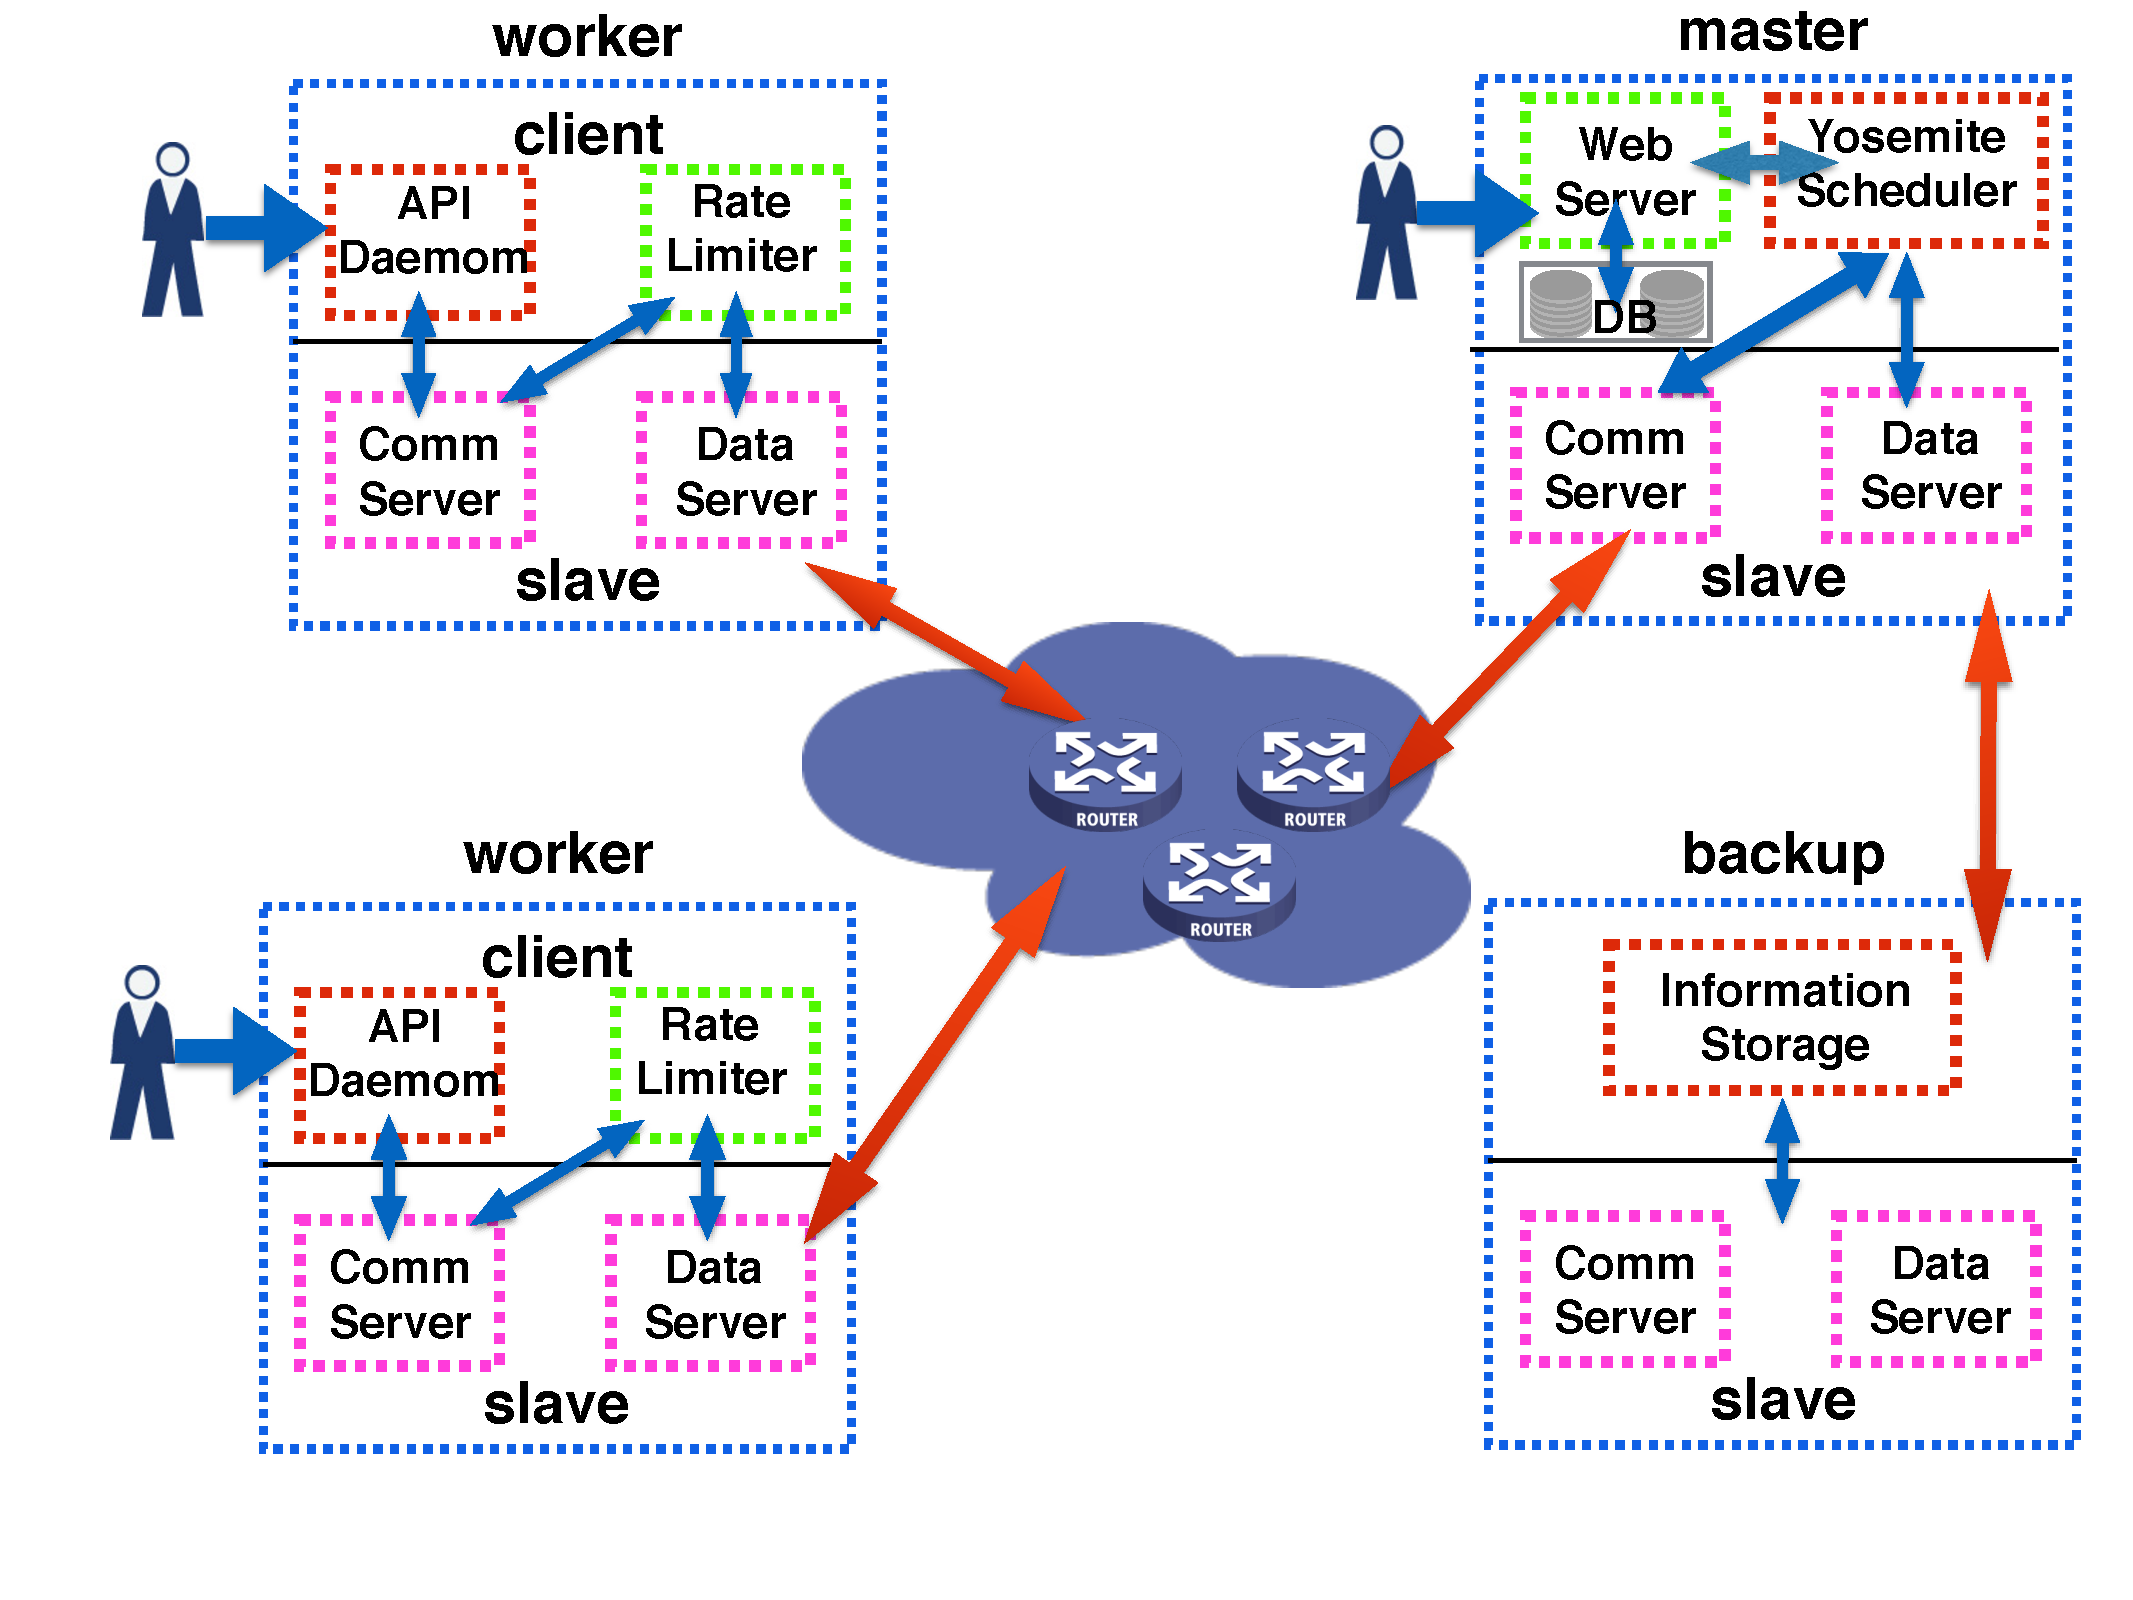
\includegraphics [width=0.8\columnwidth] {figures/Yosemite/figs/system/YosemiteSystem.pdf}
\caption{FlyTransfer 系统架构}
\label{Yosemite-design-fig}
\end{center}
\end{figure}
FlyTransfer系统包含三个组件,负责进行任务调度的master节点,
负责进行任务发送和接收的worker节点,负责进行信息备份的backup节点。
图\ref{Yosemite-design-fig}显示的是FlyTransfer系统的架构图。
其中master节点包括三个部分:和用户进行交互的UI部分-web server,
进行coflow调度的scheduler,调度器可以运行各种coflow调度算法。
进行底层通信的slave。
worker节点包含两个部分:给用户和应用提供API的client组件,底层通信slave 组件。
backup节点是进行备份,其中backup节点包括information storage和slave两个组件。
\subsection{FlyTransfer组件}
\subsubsection{master组件}
master组件是FlyTransfer系统的“大脑”部分,是整个系统的核心部分。
FlyTransfer系统采用集中式控制机制,Master节点是系统的控制部分。
master节点包括三个部分:和用户进行交互的UI部分-web server,
进行coflow调度的scheduler,调度器可以运行各种coflow调度算法。
用户可以通过Web Server查看coflow的调度实时状态,
Web Server 开放默认端口16016,其中主界面显示如图\ref{Yosemite-Master-fig}所示。
\begin{figure}[b]
\begin{center}
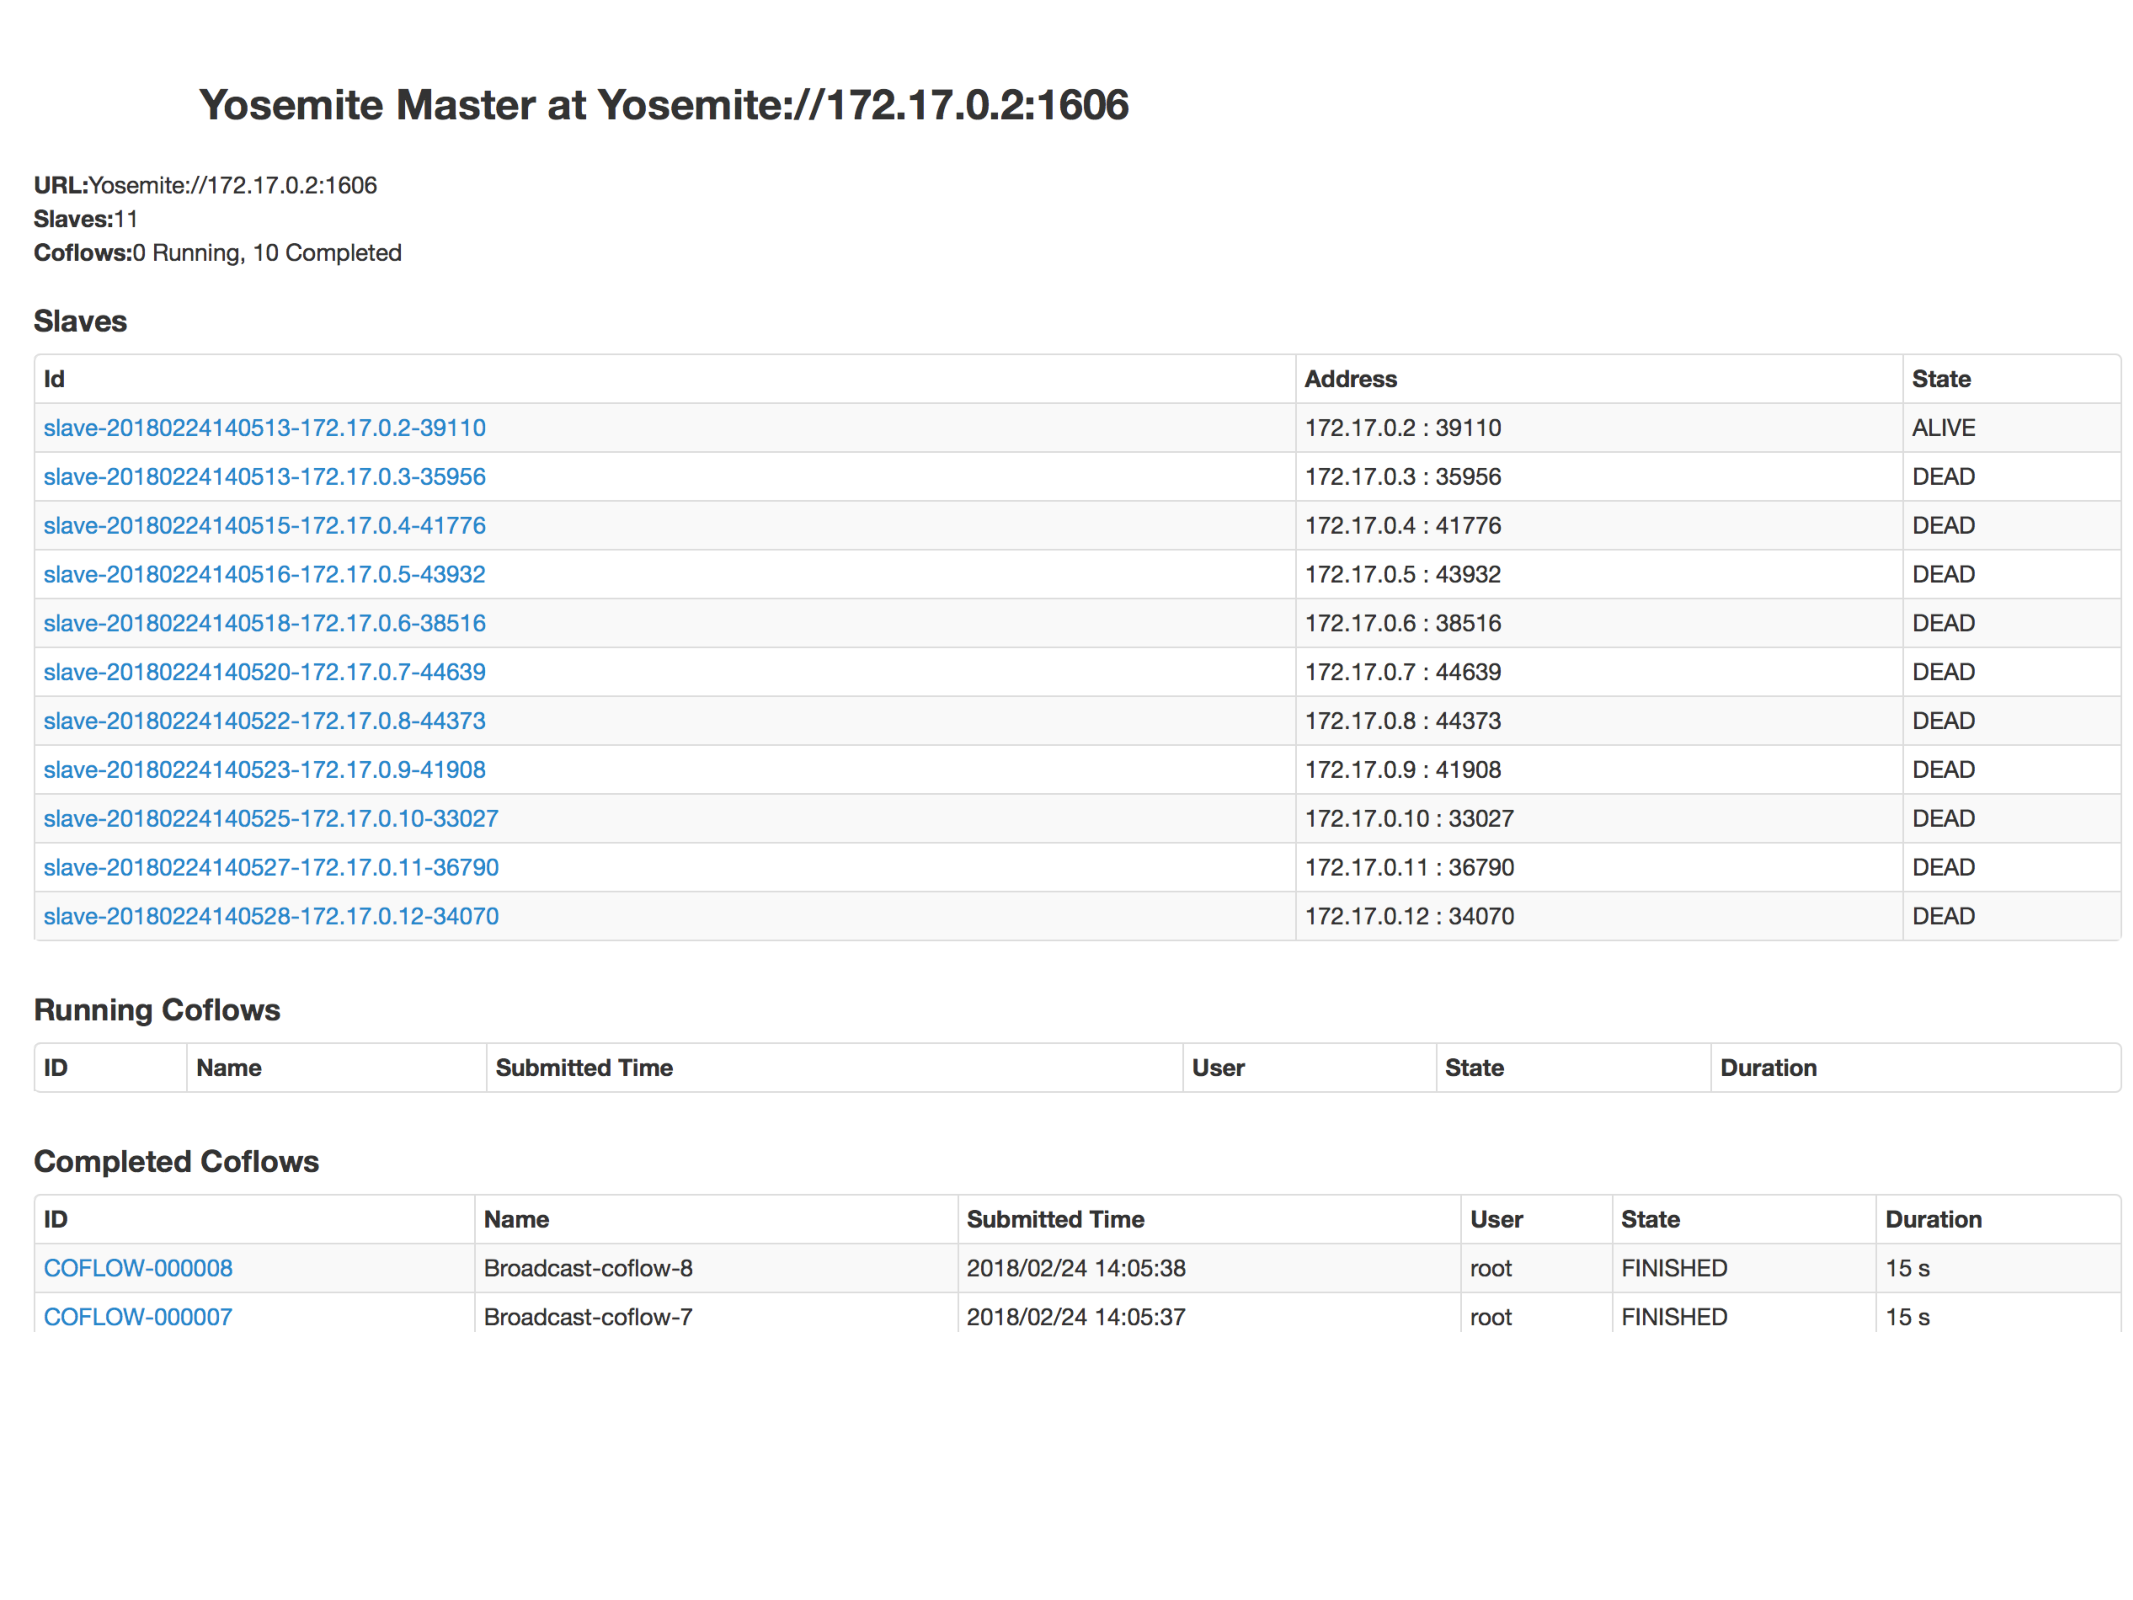
\includegraphics [width=0.8\columnwidth] {figures/Yosemite/figs/system/YosmiteMaster.pdf}
\caption{Master的UI主界面}
\label{Yosemite-Master-fig}
\end{center}
\end{figure}
\begin{figure}[h]
\centering
\subcaptionbox{Slave信息}
 {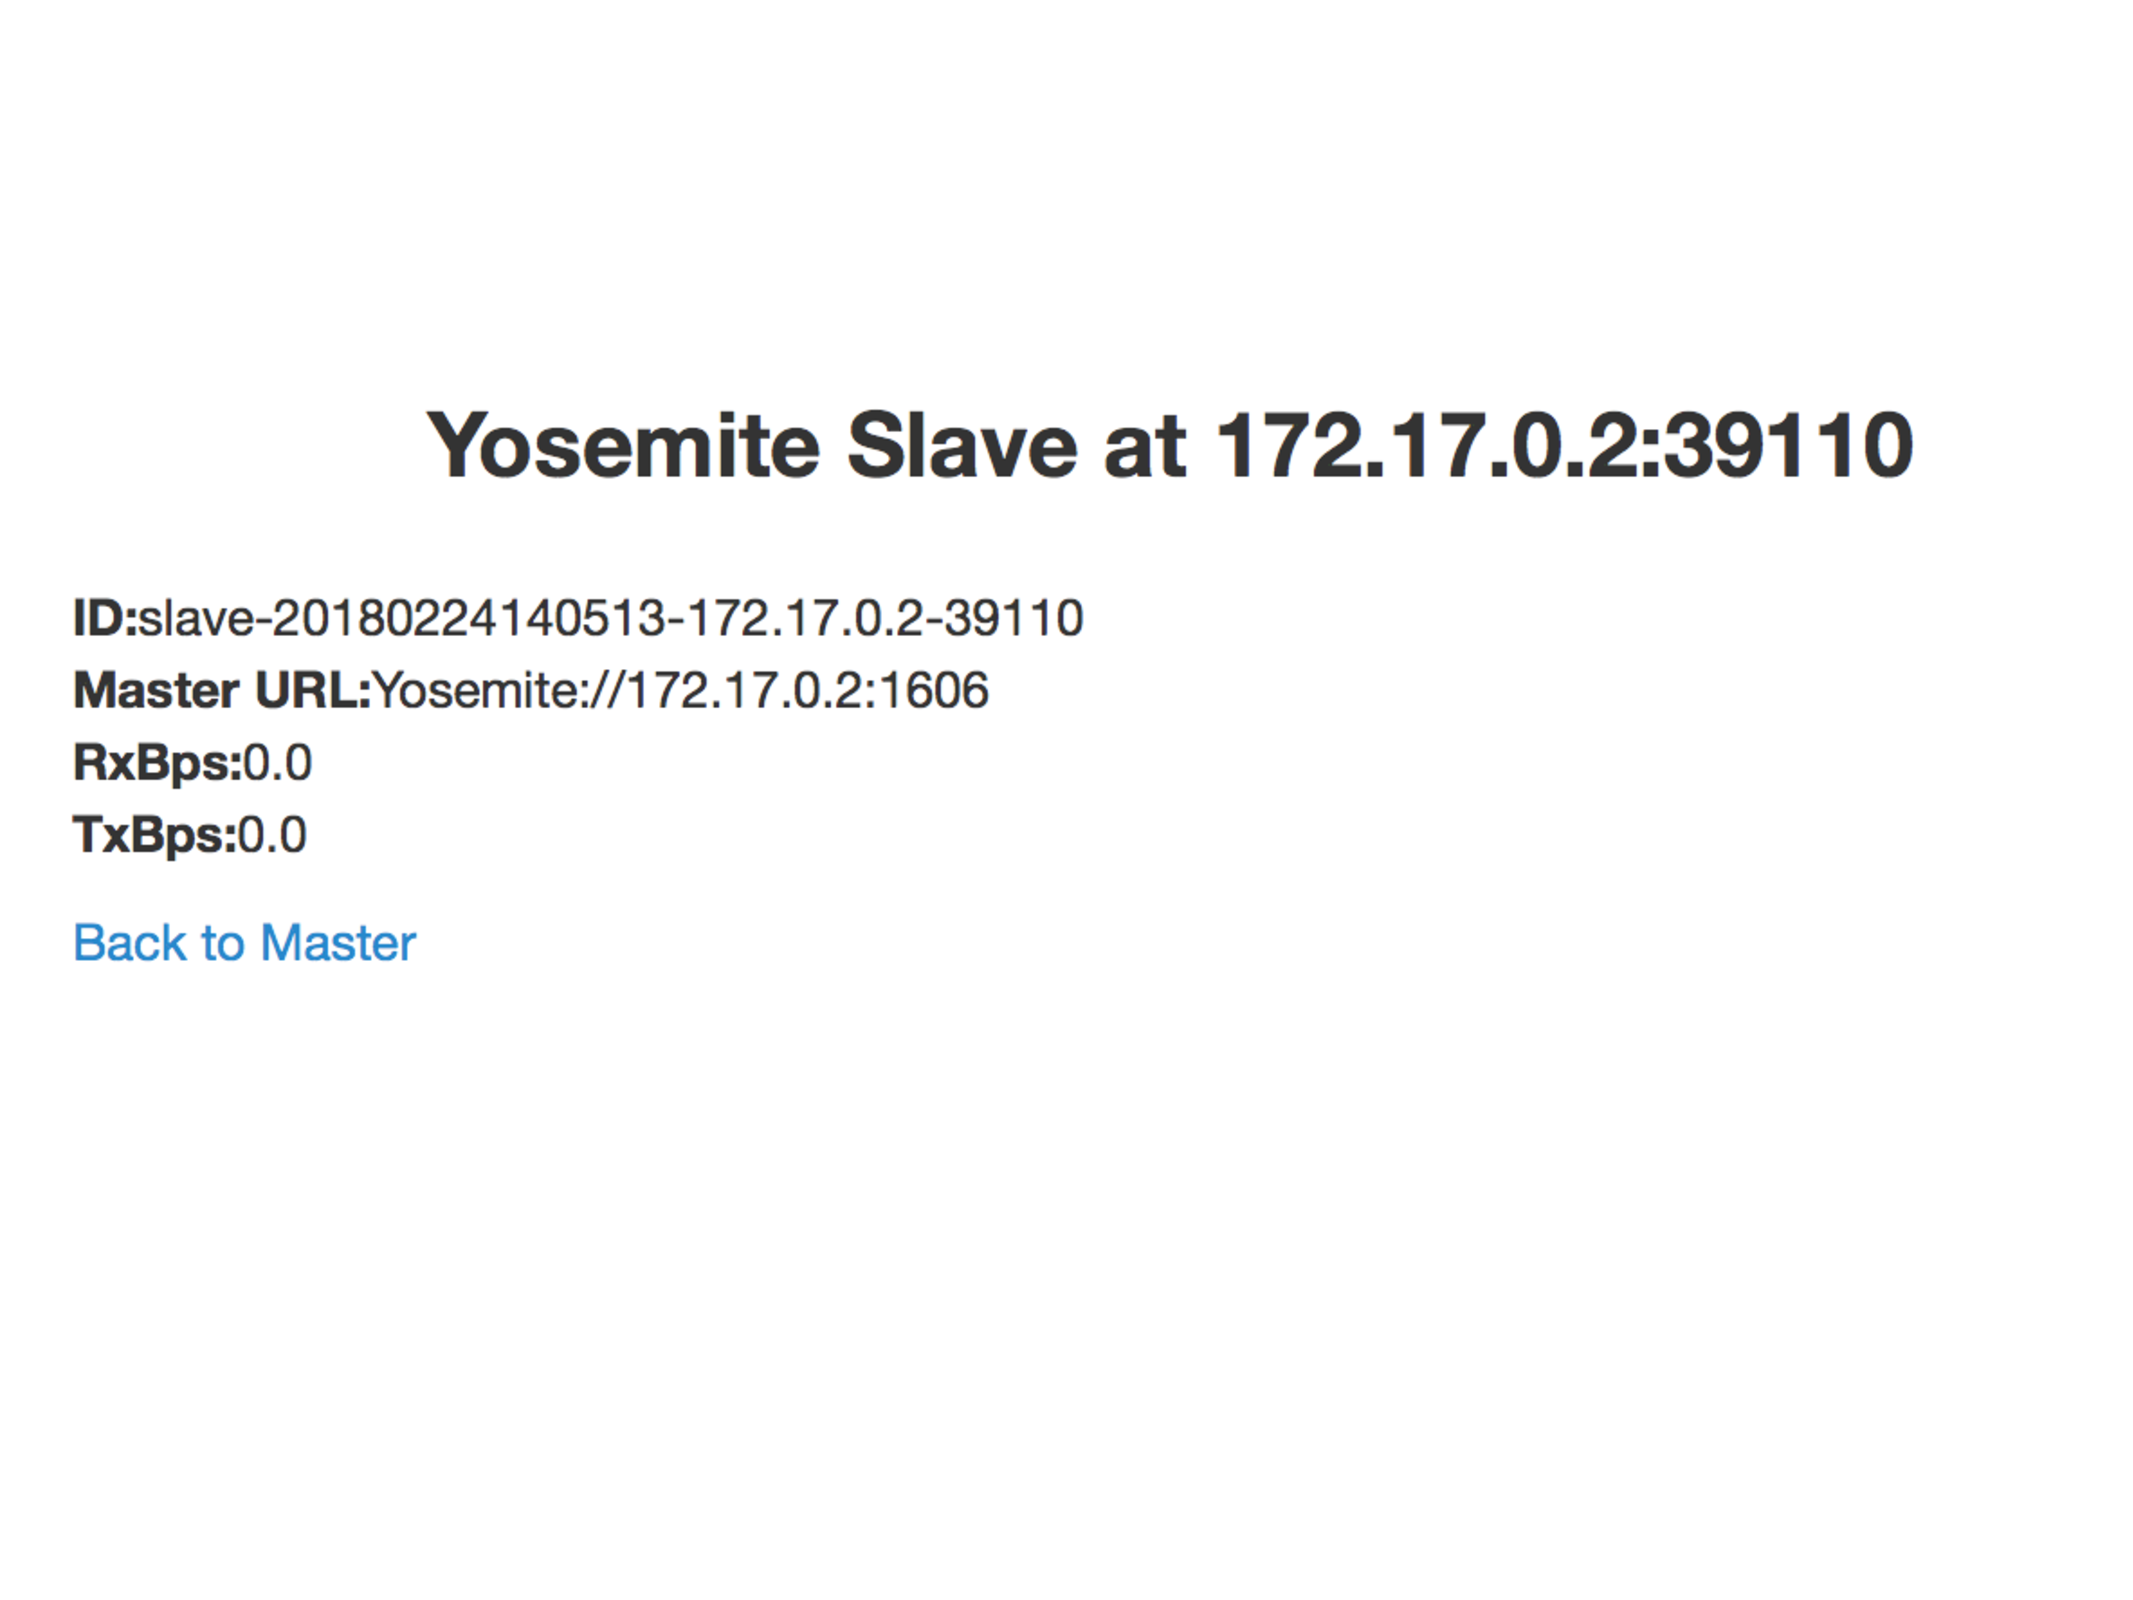
\includegraphics[width=0.48\columnwidth]{figures/Yosemite/figs/system/YosemiteSlave.pdf}}
\subcaptionbox{Coflow信息}
{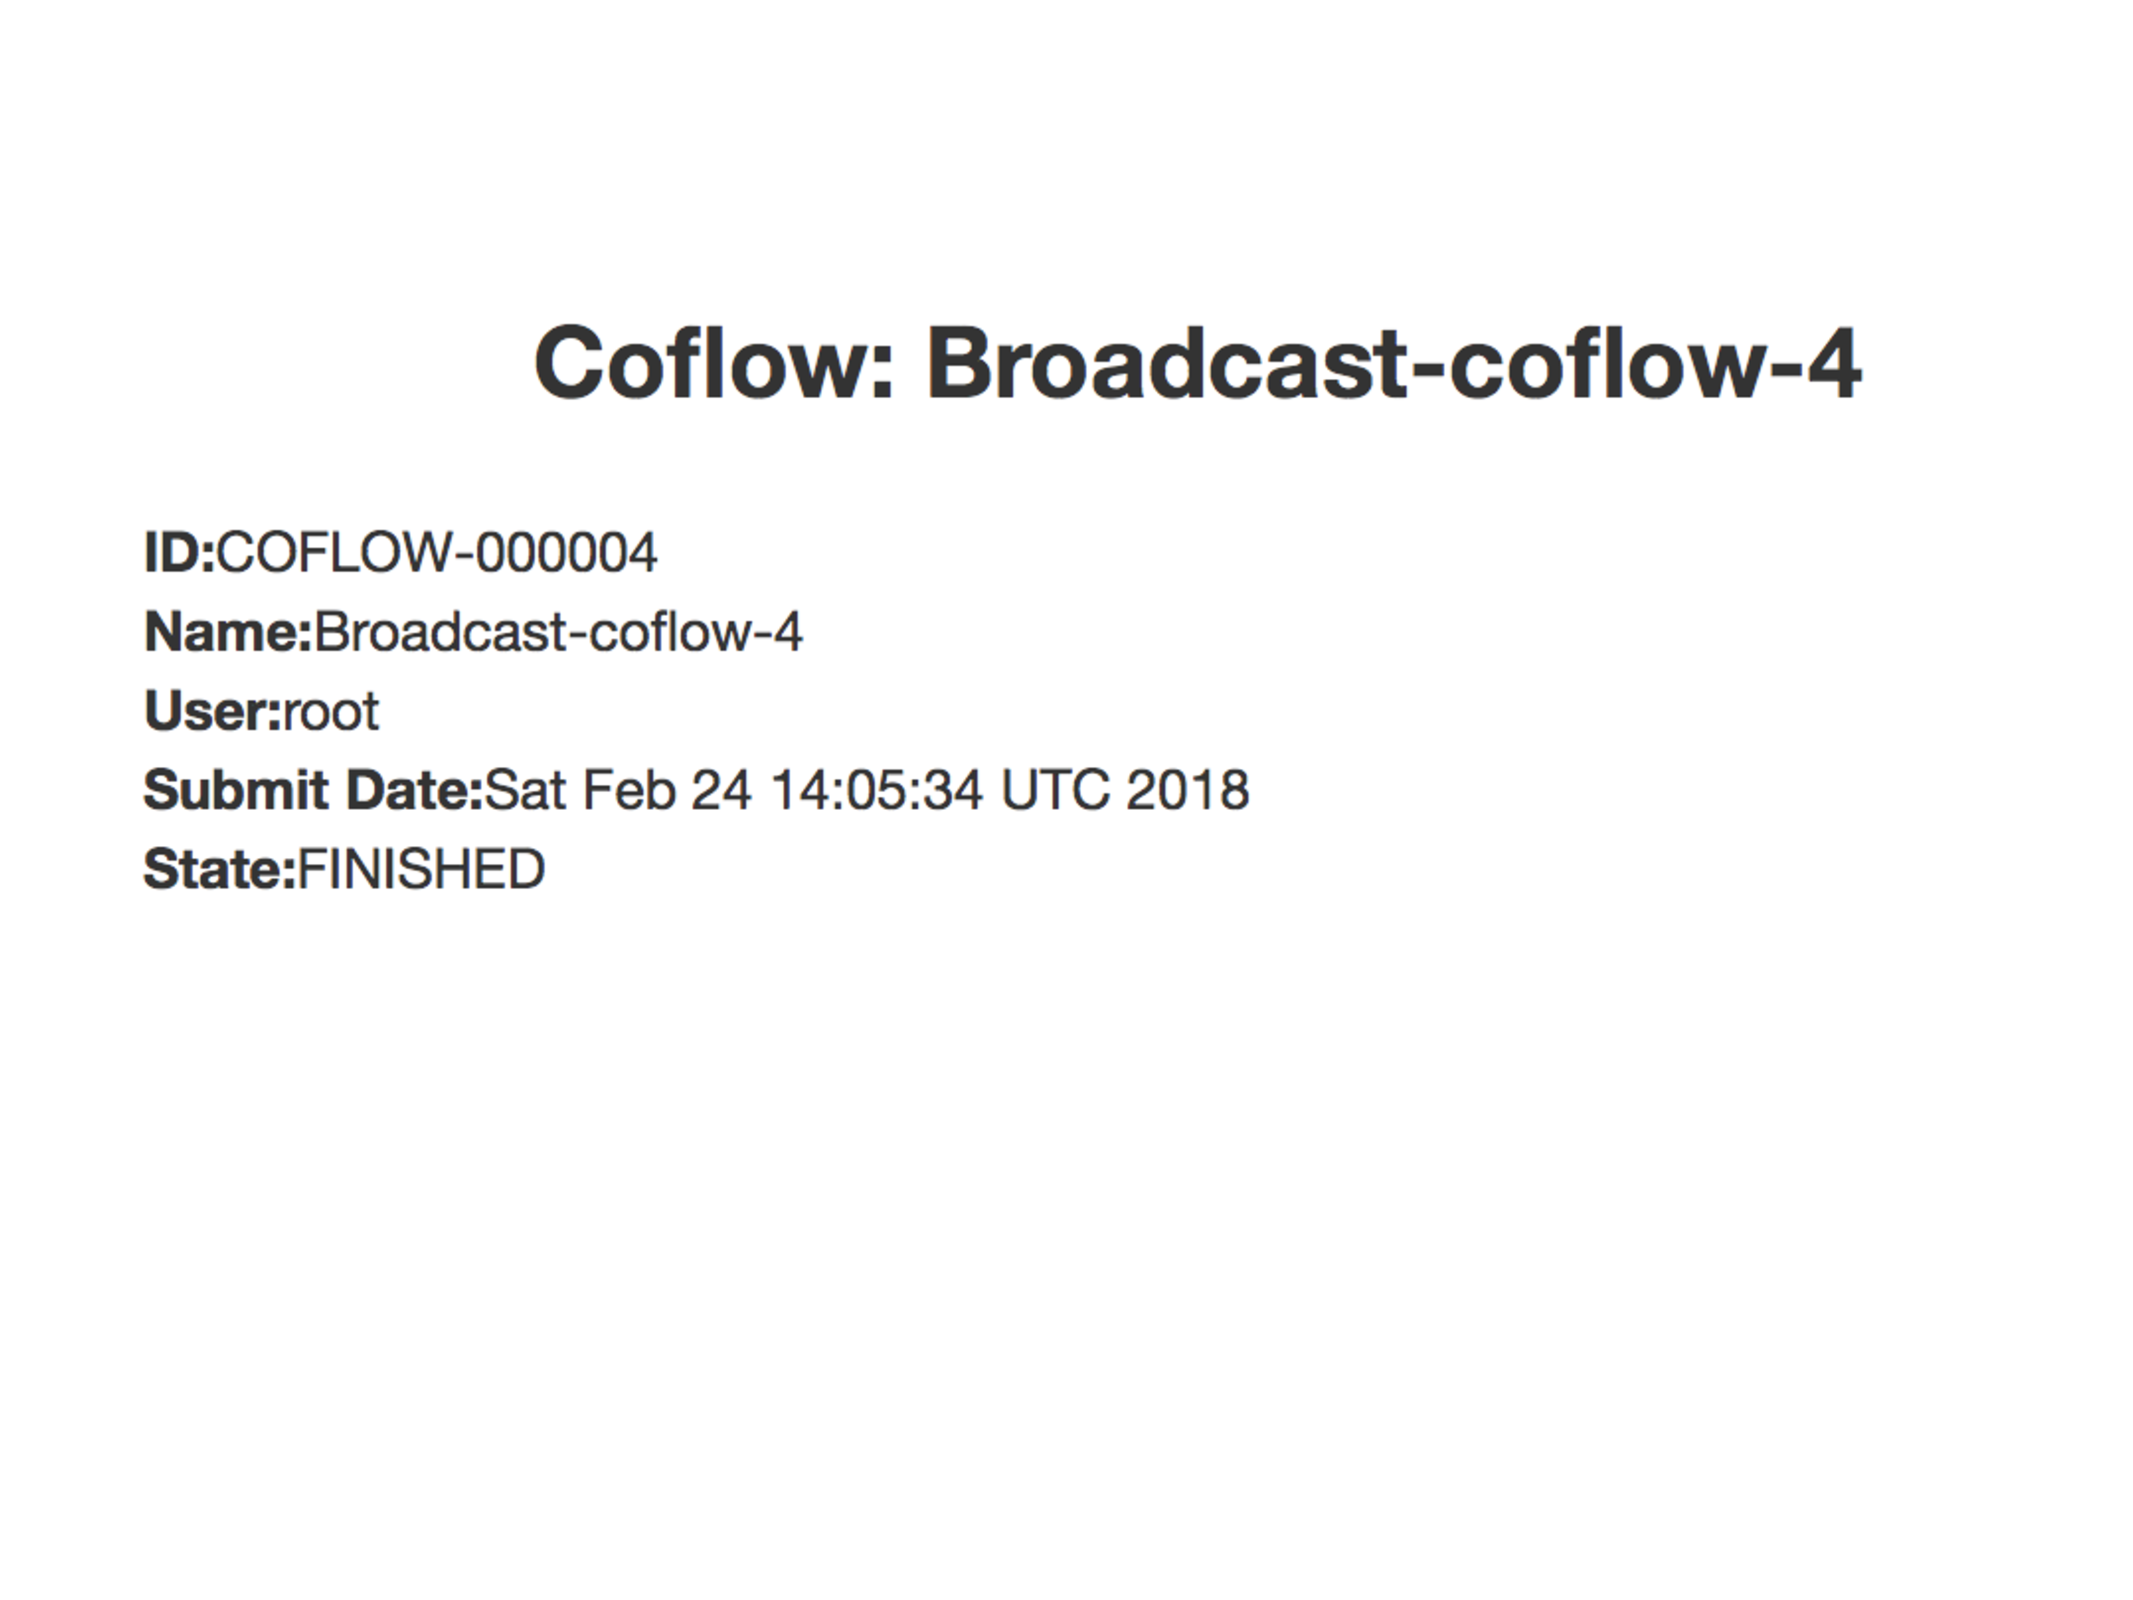
\includegraphics[width=0.48\columnwidth]{figures/Yosemite/figs/system/YosemiteCoflow.pdf}}
\caption{UI部分:Slave和Coflow}
\label{Yosemite-Salve-Coflow-fig}
\end{figure}

从图\ref{Yosemite-Master-fig}可以看到,主界面主要有三部分:
Slave的数目,正在运行coflow的信息,已经完成传输的coflow信息。
Web Server是基于jetty\footnote{http://www.eclipse.org/jetty/download.html}实现的。
Web Server同时把coflow调度的信息存储在数据库中。

图\ref{Yosemite-Salve-Coflow-fig}(a)显示的是Slave的信息,
其中包括Slave 标记(ID)和Slave的发送和接收的信息等。
图\ref{Yosemite-Salve-Coflow-fig}(b)显示的是coflow的信息,
其中包括coflow 的ID和coflow的提交时间以及coflow当前的状态(是否完成,是否在传输)等。

FlyTransfer的 Scheduler是数据中心应用数据流和任务的调度器,
在前面章节中介绍的调度策略,coflow的排序均实现在这个组件中。
本组件收集coflow的信息,并且计算每条coflow中数据流的带宽。
计算完毕后,把每条流信息传递给comm server,然后发放给对应的worker节点,
相应的worker节点按照计算的速率发送数据流。


\subsubsection{Slave组件}

Slave 负责底层通信和数据传输。Slave包括两个部分,
其中Comm Server 负责信息传递,Data Server负责数据传输。
Comm Server的信息传递是基于Akka\footnote{http://akka.io}
(Akka是JAVA虚拟机JVM平台上构建高并发、分布式和容错应用的工具包。
Akka用Scala语言写成,同时提供了Scala和JAVA的开发接口)。
使用Akka,可以有效增加系统消息的并发性能,提高系统的鲁棒性。
Comm Server 进行的信息传递如表\ref{Master:CommServer}所示。
\begin{table}[h]
\centering
\footnotesize
 \caption{Comm Server进行的信息传递} \label{Master:CommServer}
\begin{tabular}{|c|c|c|c|c|c|} \hline
\toprule
消息名称  &传输方向&说明 \\
\toprule
RegisterSlave & 从Worker到Master&注册Slave\\
\toprule
RegisteredSlave & 从Master到Worker&告知Worker,Slave注册成功\\
\toprule
RegisterSlaveFailed & 从Master到Worker&告知Worker,Slave注册失败\\
\toprule
Heartbeat & 从Worker到Master&心跳信息,判断Slave是否alive\\
\toprule
RegisterClient & 从Worker到Master&注册Client\\
\toprule
RegisteredClient & 从Master到Worker&告知Worker,Client注册成功\\
\toprule
RegisterCoflow & 从Worker到Master&注册coflow\\
\toprule
RegisteredCoflow & 从Master到Worker&注册coflow成功\\
\toprule
RegisterCoflowFailed & 从Master到Worker&注册coflow失败\\
\toprule
UnregisteredCoflow & 从Master到Worker&coflow传输完毕\\
\toprule
AddFlow & 从Worker到Master&增加数据流\\
\toprule
AddFlow & 从Worker到Master&增加一条数据流\\
\toprule
GetFlow & 从Master到Worker&获取数据流信息\\
\toprule
DeleteFlow & 从Worker到Master&删除一条数据流\\
\toprule
\end{tabular}
\end{table}
其中消息类型可以分成三类,组件的处理,coflow的处理,数据流的处理。
DataServer主要进行数据的传输,DataServer可以按照计算而得的速率进行传输。


 \subsubsection{worker组件}
 Worker节点进行数据的发送和接收,
 worker节点包含两个部分:给用户和应用提供API的client组件,
 底层通信slave 组件,其中Slave组件和Master部分相同。
 Worker节点提供的API如表\ref{Master:API}所示。
表\ref{Master:API}中API中,registerCoflow是注册coflow,其中参数为CoflowDescription,
CoflowDescription是对coflow的描述,包含coflow重要性,coflow的宽度等信息。
unregisterCoflow是注销coflow,当coflow结束传输时,此函数被调用。
handlePut参数是coflowId和flowDescription,是给系统注册一条属于coflowId的数据流。
handleGet是获得当前coflow调度的实时信息。
handleFlow是决定是否开启流级别优化,默认情况下不开启。
ChooseScheduler用来选择调度策略,默认的调度策略是Yosemite算法。

 
 \begin{table}[h]
\centering
\footnotesize
 \caption{API信息} \label{Master:API}
\begin{tabular}{|c|c|c|c|c|c|} \hline
\toprule
API名称  &参数&返回值&说明 \\
\toprule
registerCoflow&CoflowDescription&CoflowId&注册coflow,并返回coflow的Id\\
\toprule
unregisterCoflow&coflowId&boolean&注销coflow\\
\toprule
handlePut&coflowId,flowDescription&boolean&加入一条数据流\\
\toprule
handleGet&coflowId&coflowContent&得到一条coflow信息\\
\toprule
handleFlow&boolean,deadline&boolean&是否开启流级别优化,默认不开启\\
\toprule
ChooseScheduler&ScheduerId&boolean&选择要使用的调度器\\
\toprule
\end{tabular}
\end{table}
worker节点上的应用程序通过调用API来进行传输优化。
RateLimiter主要和Data Server协作,
接收来自Master计算的速率,并且按照这个计算值同Data Server共同进行速率的控制。


 \subsection{backup组件}
 backup组件是备份节点,主要进行信息备份,
 其中master组件不断的把信息传递给backup组件,
 backup组件备份正在调度的coflow的信息,同时对master组件进行监控
 当master出现宕机时,backup节点会立刻重启master组件,并且让master组件
 恢复到宕机前状态。
 
 \section{性能评估}
本部分,在私有openstack平台上部署FlyTransfer系统,并对之进行性能评估。
在openstack平台同时启动80台虚拟机(2核,4GB内存)。
每台虚拟机安装Ubuntu16.04操作系统。
在Traffic Control模块\cite{TC}的帮助下,限制每台VM网卡的带宽在1GB/s。
首先,我们进行任务级别的性能展示;
随后,是流级别的性能评估。
最后,我们对系统的开销进行评估。

 \subsection{任务级优化对比}

\begin{figure}[h]
  \centering%
  \subcaptionbox{平均CCT} %标题的长度,超过则会换行,如下一个小图。
    {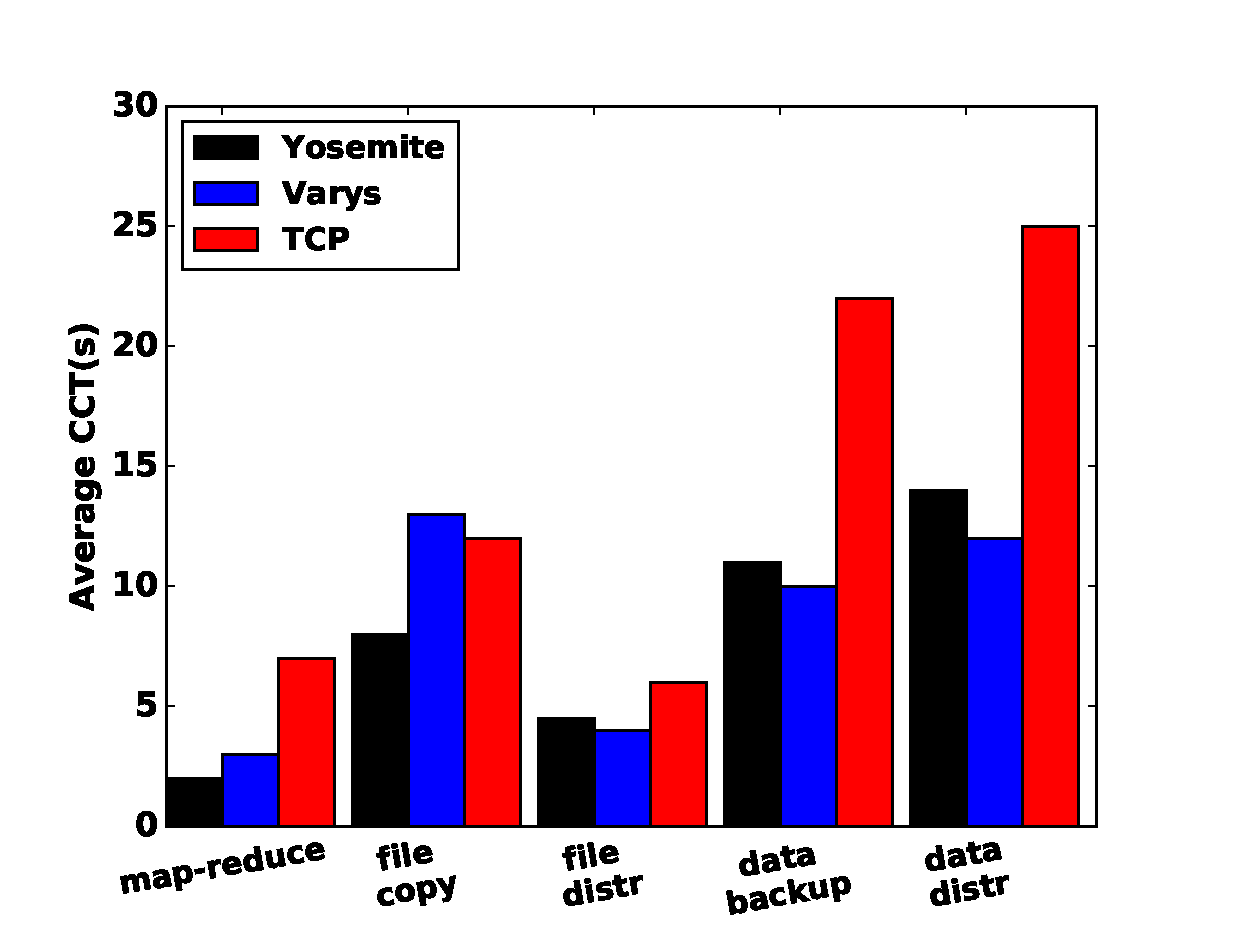
\includegraphics[width=0.5\columnwidth]{figures/Yosemite/figs/evaluation/ex5/real1.eps}}%
  \subcaptionbox{平均CCT(95th)}
      {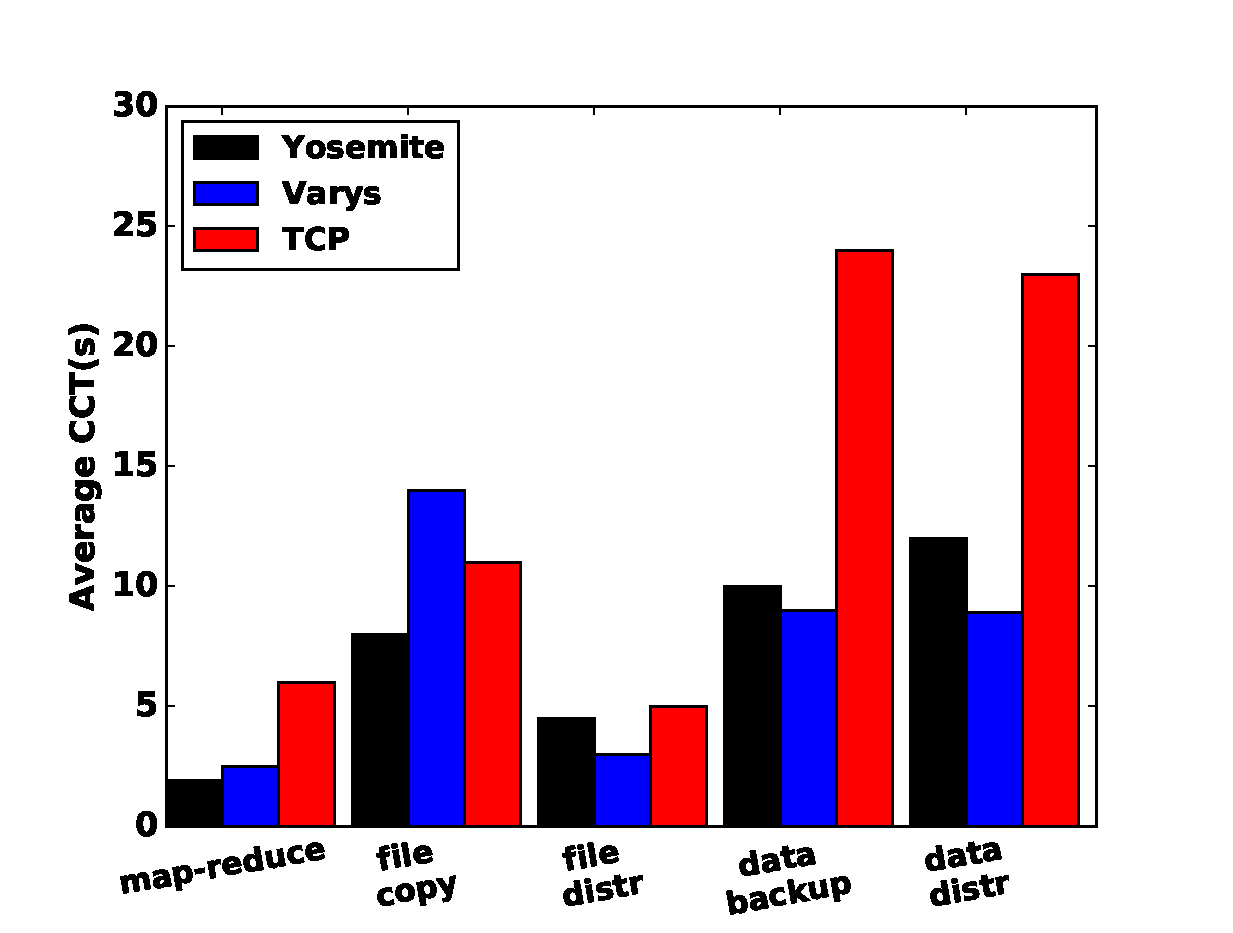
\includegraphics[width=0.5\columnwidth]{figures/Yosemite/figs/evaluation/ex5/real2.eps}}
  \subcaptionbox{Hadoop CCT}%标题的长度,超过则会换行,如下一个小图。
    {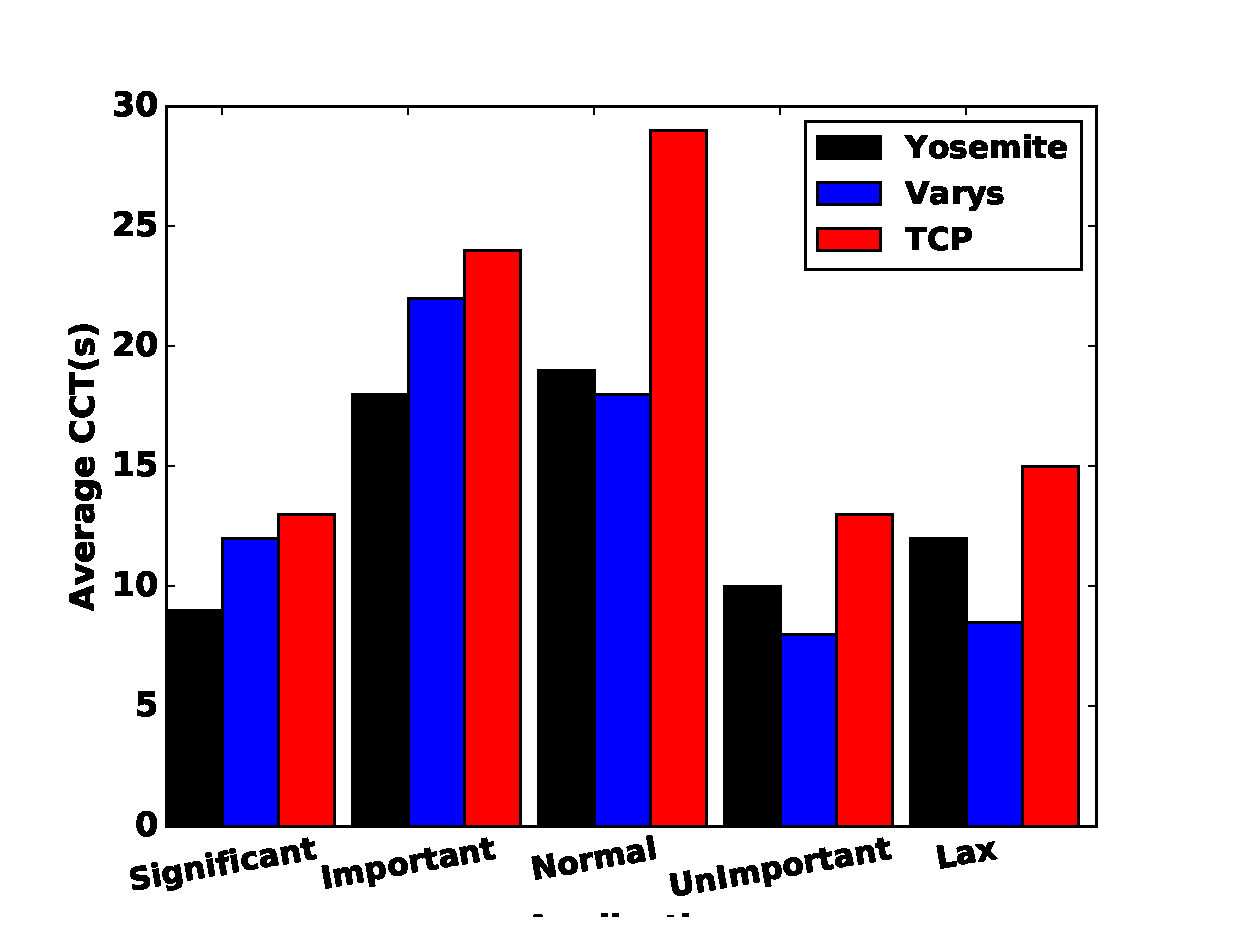
\includegraphics[width=0.5\columnwidth]{figures/Yosemite/figs/evaluation/ex5/real3.eps}}%
  %\hspace{7em}%
  \subcaptionbox{Hadoop CCT (95th)}
      {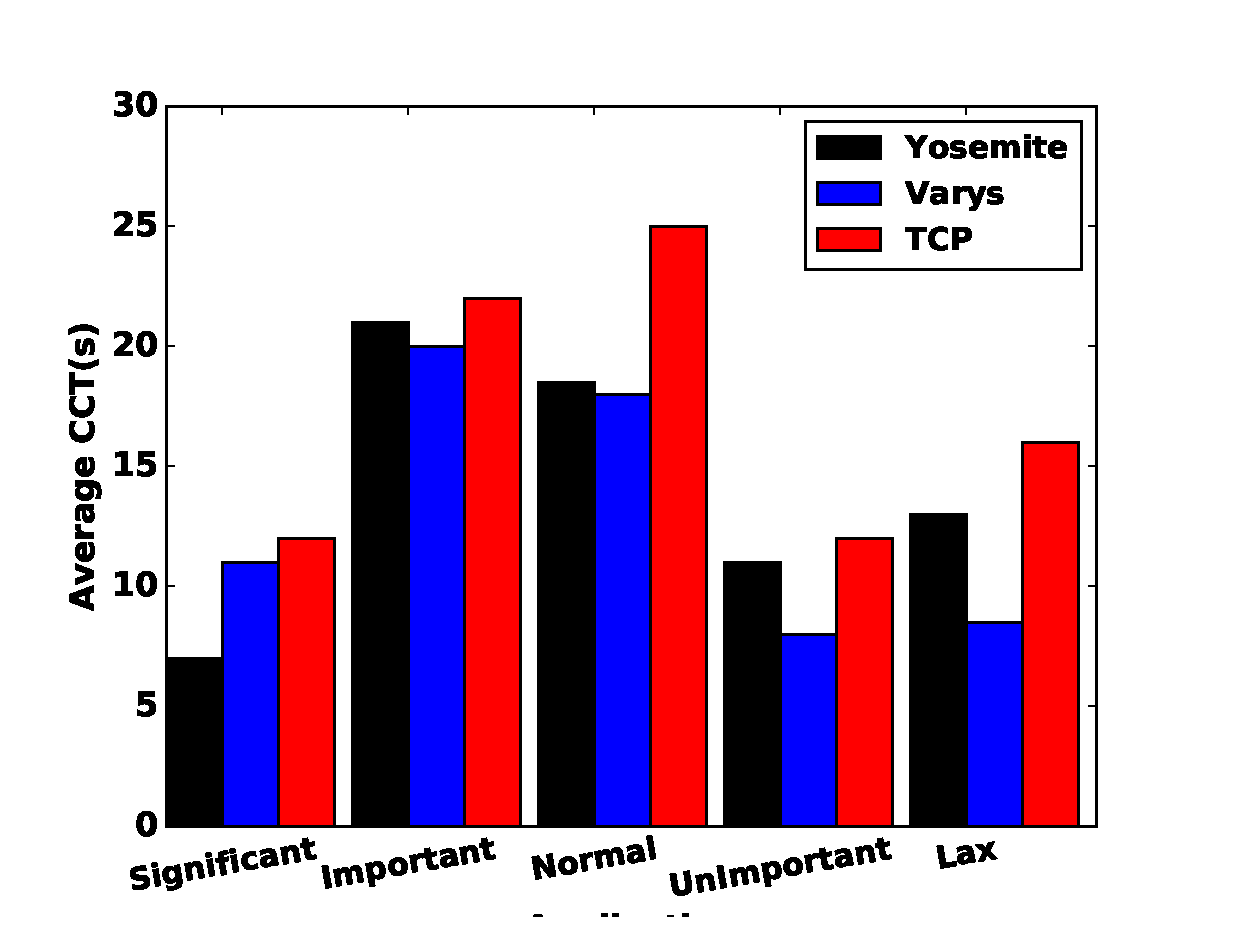
\includegraphics[width=0.5\columnwidth]{figures/Yosemite/figs/evaluation/ex5/real4.eps}}
  \caption{[真实测试] openstack 真实环境下不同应用的测试}
  \label{Yosemite-evaluation_cloud_fig}
\end{figure}
选择FlyTransfer任务调度策略是Yosemite,并在数据中心中部署5个应用: map-reduce, file-copy, file-distribute, data-backup, data-distribute。
这5个应用的优先级分别是紧急,重要,正常,不重要,松散。
图\ref{Yosemite-evaluation_cloud_fig}(a)是整体的平均CCT实验结果,从实验结果看,
使用使用FlyTransfer使用Yosemite策略下的下的map-reduce, file-copy, file-distribute, data-backup, data-distribute,5类应用的平均CCT分别为:2,7,4,10,12。
使用Varys下的map-reduce, file-copy, file-distribute, data-backup, data-distribute,5类应用的平均CCT分别为:3,14,3,9,11。
使用TCP,这5类应用的平均CCT分别为:7,12,6,22,25。
为了避免某些极端值对实验结论的影响,我们绘制了95th比例coflow的平均CCT实验结果,如图\ref{Yosemite-evaluation_cloud_fig}(b)所示。
我们发现使用FlyTransfer使用Yosemite策略下的map-reduce, file-copy, file-distribute, data-backup, data-distribute,5类应用的平均CCT分别为1.9,6,3,9.4,13。
使用Varys结果是:3.1,13,2.4,9.2,10。
使用TCP,这5类应用的平均CCT分别为:6.8,11.2,5,21,23。
我们看到对于重要的应用map-reduce, file-copy,使用FlyTransfer使用Yosemite策略下的性能比Varys提高20\% $ \sim$ 30\%,但是对于不重要的应用,使用FlyTransfer使用Yosemite策略下的性能比Varys性能差20\%。图\ref{Yosemite-evaluation_cloud_fig}(c)展示的是file-distribution的结果,给应用的coflow设置5个优先级:紧急,重要,正常,不重要,松散,我们发现Yosemite性能比Varys提高 20\%,图\ref{Yosemite-evaluation_cloud_fig}(d) 的结果类似。

 \subsection{流级优化对比}
 \begin{figure}[h]
  \centering%
  \subcaptionbox{紧急期限(20ms)} %标题的长度,超过则会换行,如下一个小图。
      {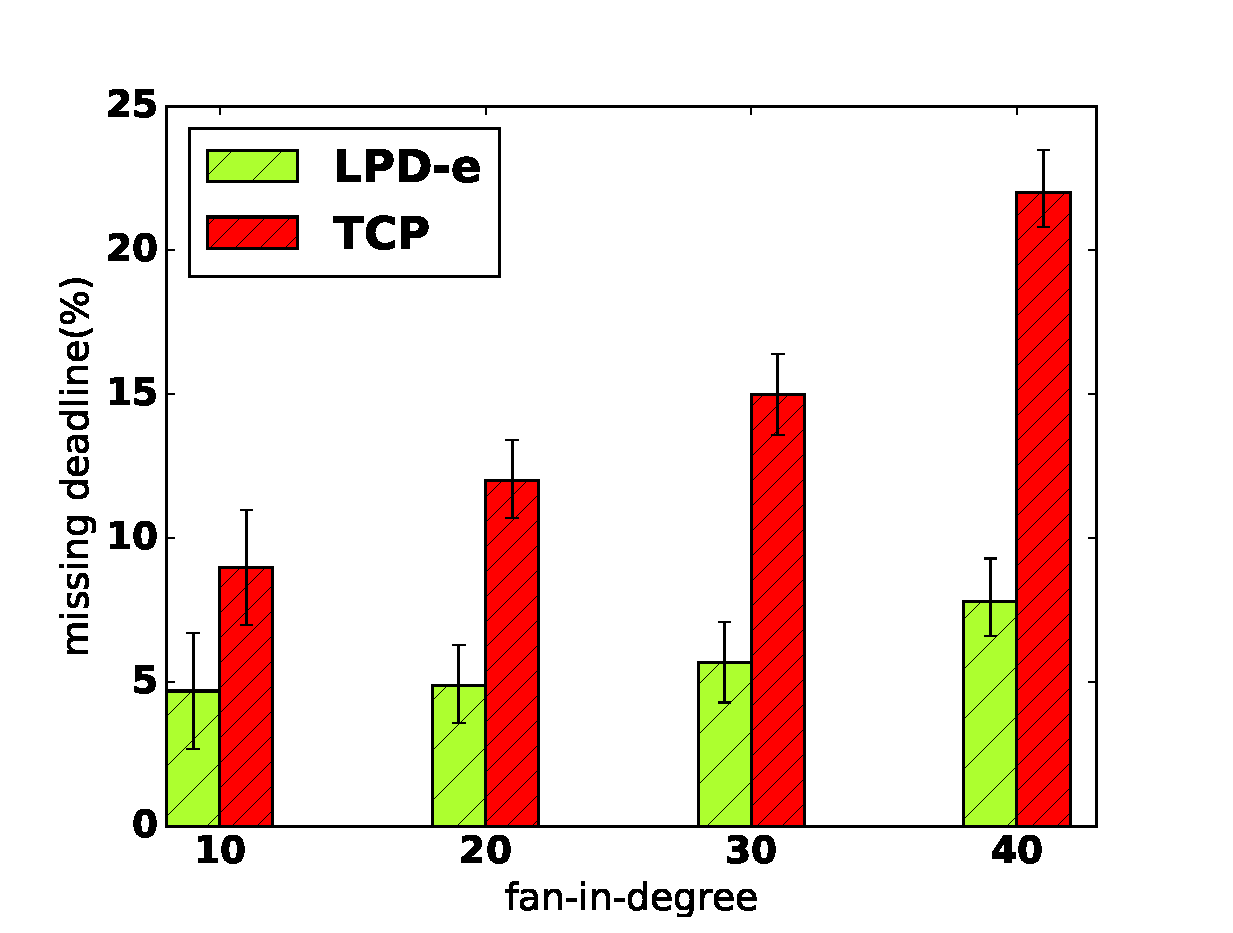
\includegraphics[width=0.33\columnwidth]{figures/others/20ms.eps}}
  \subcaptionbox{中等期限(30ms)}%标题的长度,超过则会换行,如下一个小图。
    {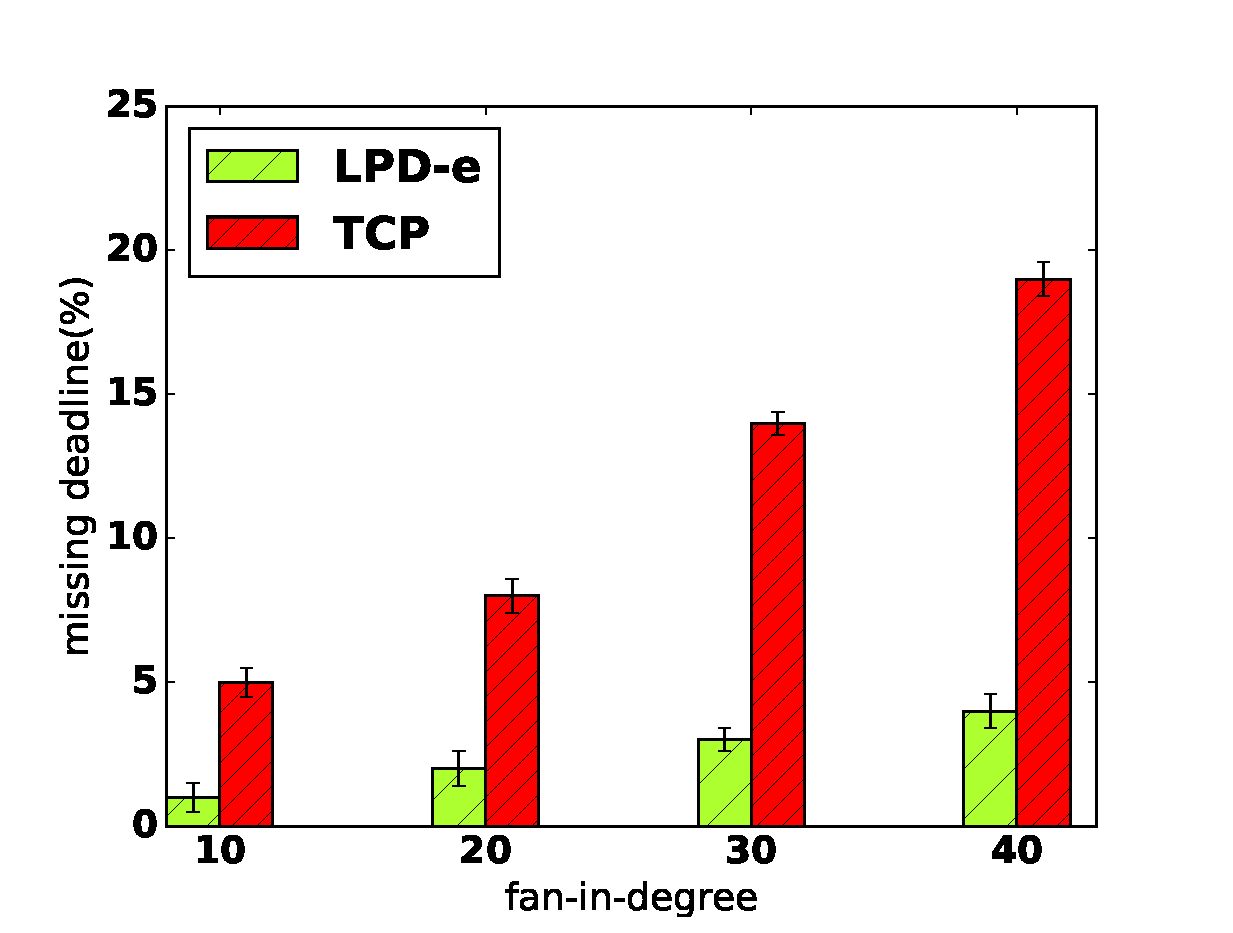
\includegraphics[width=0.33\columnwidth]{figures/others/30ms.eps}}%
      \subcaptionbox{松弛期限(40ms)}%标题的长度,超过则会换行,如下一个小图。
    {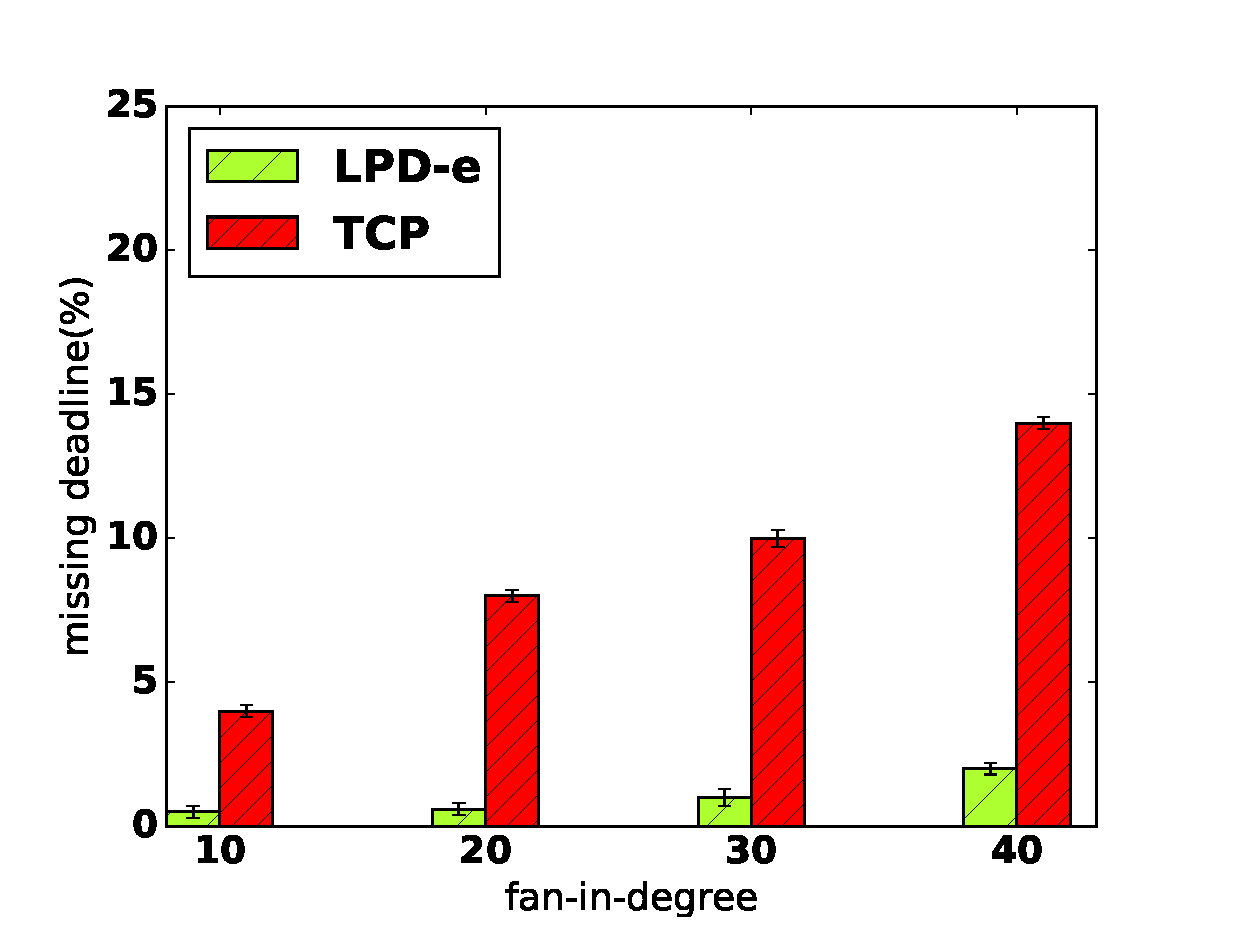
\includegraphics[width=0.33\columnwidth]{figures/others/40ms.eps}}%

  %\hspace{7em}%
   \caption{[真实测试] 错失期限对比}
  \label{Yosemite-evaluation_deadline_fig}
\end{figure}

 图\ref{Yosemite-evaluation_deadline_fig}展示错失期限对比。
 开启对流优化的API,在openstack中构建OLDI场景,数据流发送服从柏松分布,
 假设期限服从指数分布。
 流的期限平均设置为紧急期限(20ms),中等期限(30ms)和松弛期限(40ms)。
 从图\ref{Yosemite-evaluation_deadline_fig}(a)可以看到,当紧急期限为20ms时,
 当fan-in-degree从10到40时,LPD-e下错失期限的比例分别为5$\%$,6$\%$,7$\%$,8$\%$。
 而使用TCP错失期限的比例分别为9$\%$,12$\%$,14$\%$,22$\%$。
 LPD-e的性能比TCP平均提高2.5$\times$。
 对于中等期限(30ms)和松弛期限(40ms),从图\ref{Yosemite-evaluation_deadline_fig}(b)和从图\ref{Yosemite-evaluation_deadline_fig}(c)可以看到,结果和紧急期限(20ms)时类似。
 
 
 \subsection{系统开销}
 \begin{figure}[h]
  \centering%
  \subcaptionbox{并行coflow影响} %标题的长度,超过则会换行,如下一个小图。
      {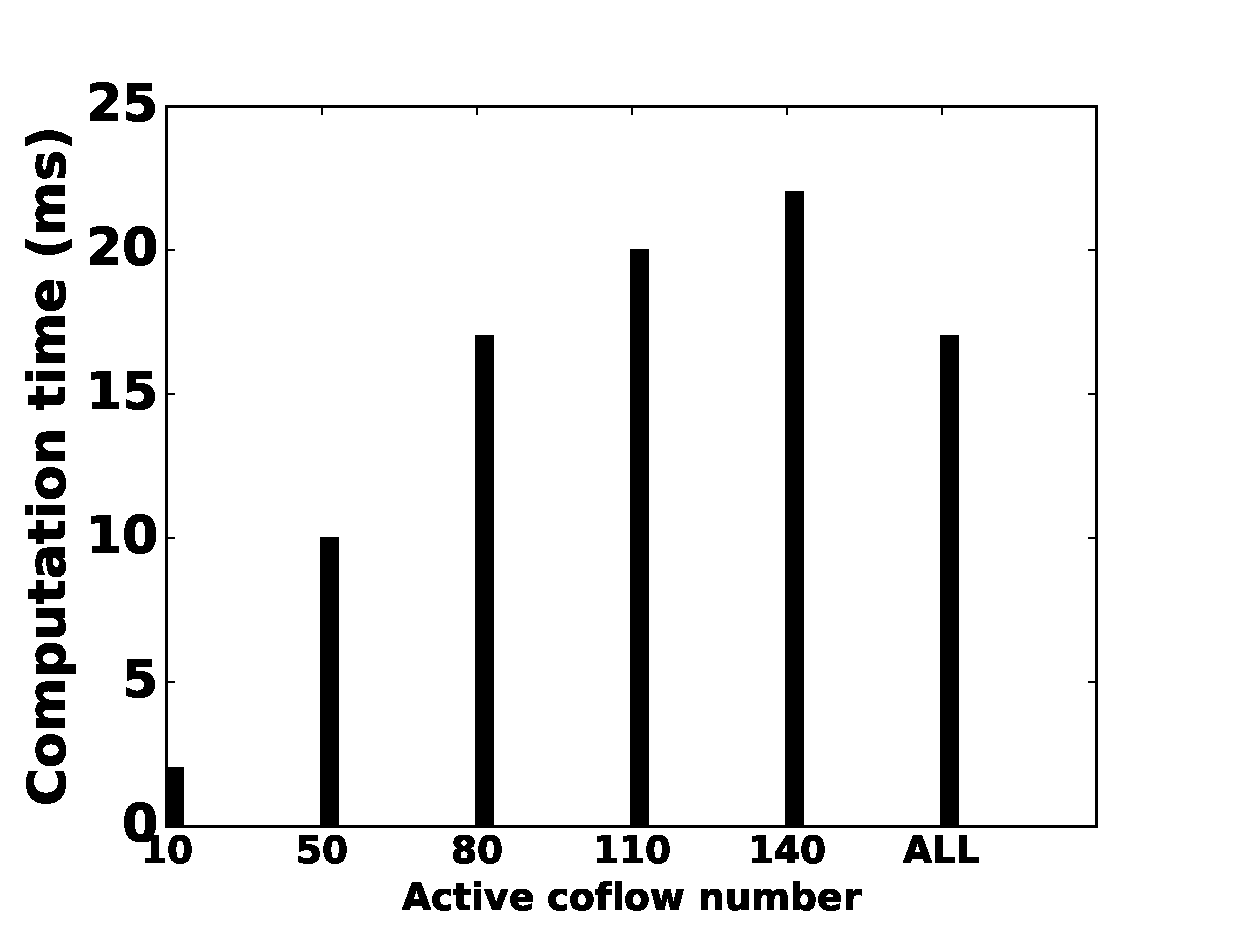
\includegraphics[width=0.49\columnwidth]{figures/Yosemite/figs/fake/fake5.eps}}
  \subcaptionbox{错误消息}%标题的长度,超过则会换行,如下一个小图。
    {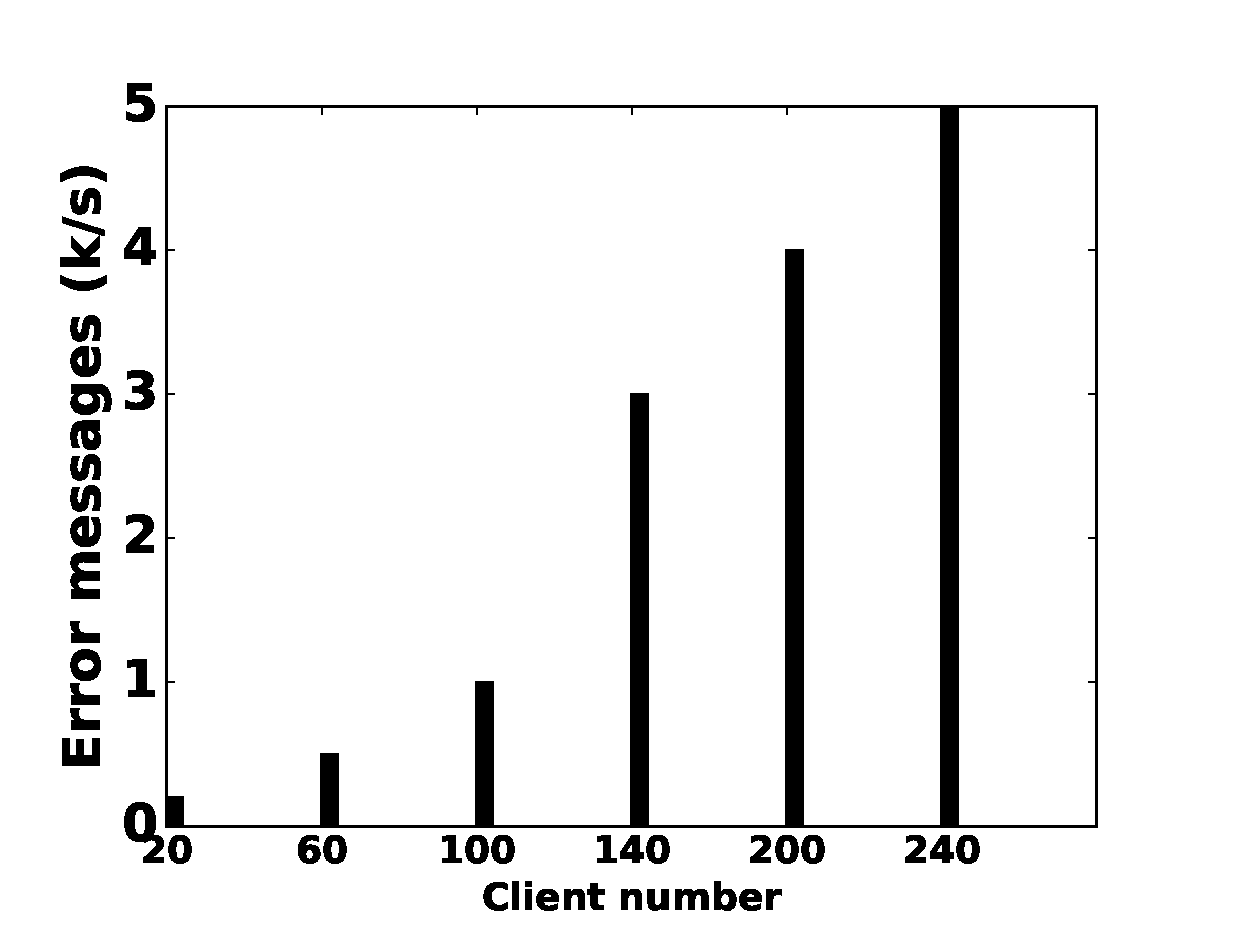
\includegraphics[width=0.49\columnwidth]{figures/Yosemite/figs/fake/fake6.eps}}%
  %\hspace{7em}%
   \caption{[真实测试] FlyTransfer的开销}
  \label{Yosemite-evaluation_overhead_fig}
\end{figure}
 图\ref{Yosemite-evaluation_overhead_fig}表示的是FlyTransfer的系统开销。
 在实际中,随着并行任务和数据流的增多,控制器的计算时间增大。
 随着client组件增加,产生出错误消息会增加。
 图\ref{Yosemite-evaluation_overhead_fig}(a)展示的是随着并行任务的增加,控制器的计算时间,
 可以看到,当并行任务在140时,控制器计算时间大约是22ms,当并行任务从10ms增到140ms时,平均计算时间是18ms。
 图\ref{Yosemite-evaluation_overhead_fig}(b)展示的是随着client组件增加,并行任务的错误消息情形。
 可以看到,当client数目在240时,错误消息比例是5k/s,对比Varys系统,错误消息为6k/s,
 因此,可以看到Yosemite因为错误消息造成的开销比Varys小。

\section{本章小结}
本章对数据中心传输系统Fly-Transfer进行了介绍,首先,本章对Fly-Transfer整体架构进行了介绍,
然后本章介绍了Fly-Transfer的各个组件,最后,本章从任务调度,流传输以及系统开销方面对Fly-Transfer进行了性能评估。


 








